\section{Database Design and Storage}
\label{sec:database}

\subsection{Choice of database engine}

The master panel is stored in a single SQLite file,
\texttt{dsm\_project.db}, which weighs 577 KB on disk and contains one
table, \texttt{Weekly\_Macro\_Master}, with 545 rows and 119 columns.
SQLite was chosen over a server database for four practical reasons:

\begin{itemize}
\item Zero configuration. No separate server process is required, and
  the database file can be embedded directly into the FastAPI process
  on Render.
\item File portability. The 577 KB database is committed to the git
  repository, which means an evaluator can clone the repo, run the
  backend, and reproduce every figure without re-running any pipeline.
\item Sufficient capacity. A 545-row by 119-column panel is far below
  the threshold at which SQLite ceases to perform well; queries return
  in single-digit milliseconds.
\item Tooling support. The standard Python \texttt{sqlite3} library
  ships with the runtime, and the \texttt{sqlite-utils} CLI provides a
  convenient inspection layer during development.
\end{itemize}

The pipeline never updates rows in place. Each stage rebuilds the
table from its source CSV, which makes the database idempotent and
makes debugging straightforward.

\subsection{Schema}

\begin{figure}[H]
\centering
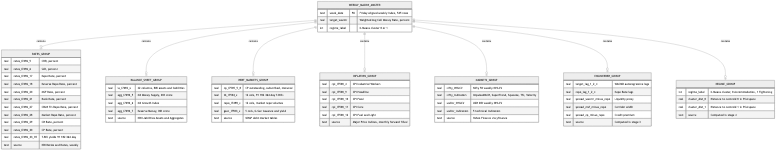
\includegraphics[width=\linewidth]{../diagram/db_schema.png}
\caption{Logical entity grouping of \texttt{Weekly\_Macro\_Master}.
Columns are organised into seven thematic groups by source family.
The actual physical schema is a single flat table; the grouping is
logical and is enforced by column-name prefixes.}
\label{fig:db-schema}
\end{figure}

The physical schema is intentionally flat. Each row is one Friday-aligned
week, indexed by \texttt{week\_date}. Columns are grouped by source
family through a deliberate naming convention: \texttt{rates\_*} for
the corridor and rate columns, \texttt{la\_*} for liabilities and
assets, \texttt{agg\_*} for aggregates, \texttt{cp\_*} for commercial
paper, \texttt{tb\_*} for Treasury Bills, \texttt{repo\_*} for market
repo, \texttt{gsec\_*} for G-Secs, \texttt{cpi\_*} for inflation,
\texttt{nifty\_*} and \texttt{usdinr\_*} for the supplemental market
data, plus \texttt{regime\_label} and \texttt{cluster\_dist\_*} from
Stage 4. The target variable lives in \texttt{target\_wacmr}, which is
a copy of \texttt{rates\_I7496\_26} from the RBI Ratios and Rates
table, retained as a separate column so that the modelling code can
treat the target uniformly without having to know its NDAP provenance.

\subsection{Friday-alignment design}

The eight NDAP datasets use three different temporal index conventions:
calendar dates as ISO-8601 strings, financial-year week codes (where
week 1 starts on April 1), and calendar-year week codes (where week 1
starts on January 1). A single naive \texttt{pd.to\_datetime} call
silently produces dates that are off by up to twelve weeks for the
financial-year tables. Three separate parsing functions were written,
one per format, each of which decodes the source date and snaps it to
the nearest following Friday. The Friday is the canonical weekly
anchor used elsewhere in the panel.

The Yahoo Finance OHLCV series are themselves anchored to different
weekdays (Nifty 50 is Monday-indexed by NSE convention; USD/INR
appears Wednesday-indexed in some weeks). Both are explicitly
resampled with \texttt{resample("W-FRI")} before computing technical
indicators, which produces a single 552-row series per instrument that
joins cleanly to the NDAP master.

\subsection{Representative analytical queries}

Four representative SQL queries below show how the database supports
the rest of the analysis. Each query was used in production to
generate either a chart or a number cited in this report.

\subsubsection*{Q1. Regime-stratified means of corridor variables}

\textbf{Question.} What are the mean policy rates inside each
discovered monetary regime?

\textbf{Methodology.} Group by the \texttt{regime\_label} column
(populated by Stage 4 from the K-Means fit) and compute the mean of
the three corridor rates plus the WACMR target.

\begin{lstlisting}[style=sql,caption={Q1, regime-stratified policy-rate means.}]
SELECT
  regime_label,
  COUNT(*)                         AS weeks,
  ROUND(AVG(target_wacmr),    3)   AS avg_wacmr,
  ROUND(AVG(rates_I7496_17),  3)   AS avg_repo,
  ROUND(AVG(rates_I7496_18),  3)   AS avg_reverse_repo,
  ROUND(AVG(rates_I7496_20),  3)   AS avg_msf
FROM Weekly_Macro_Master
GROUP BY regime_label
ORDER BY regime_label;
\end{lstlisting}

\textbf{Result.} Regime 1 (315 weeks) has mean WACMR 6.528\%, mean
Repo 6.591\%, and mean MSF 7.149\%. Regime 0 (230 weeks) has mean
WACMR 4.809\%, mean Repo 5.119\%, and mean MSF 5.369\%. The 1.72
percentage-point spread between the two regime means is itself a
quantitative confirmation that the cluster boundary corresponds to a
real macroeconomic regime change rather than to a statistical artefact.

\subsubsection*{Q2. Monthly volatility of WACMR versus Repo}

\textbf{Question.} How volatile is WACMR within each calendar month
relative to the policy Repo Rate, and is the answer different across
regimes?

\begin{lstlisting}[style=sql,caption={Q2, monthly within-period volatility.}]
WITH monthly AS (
  SELECT
    SUBSTR(week_date, 1, 7)          AS yyyymm,
    regime_label,
    target_wacmr,
    rates_I7496_17                    AS repo
  FROM Weekly_Macro_Master
)
SELECT
  regime_label,
  ROUND(AVG(stddev_wacmr), 4) AS avg_within_month_wacmr_vol,
  ROUND(AVG(stddev_repo),  4) AS avg_within_month_repo_vol
FROM (
  SELECT
    yyyymm,
    regime_label,
    -- SQLite has no STDDEV; emulate via sqrt of variance over month buckets.
    SQRT(AVG(target_wacmr*target_wacmr) - AVG(target_wacmr)*AVG(target_wacmr)) AS stddev_wacmr,
    SQRT(AVG(repo*repo)               - AVG(repo)*AVG(repo))                   AS stddev_repo
  FROM monthly
  GROUP BY yyyymm, regime_label
)
GROUP BY regime_label;
\end{lstlisting}

\textbf{Result.} WACMR within-month volatility is 0.178 percentage
points in Regime 0 and 0.083 in Regime 1. The Repo Rate is essentially
constant within a month in both regimes. The doubling of WACMR
volatility in Regime 0 reflects RBI's discretionary VRR/VRRR
operations, which inject and absorb liquidity at irregular intervals
and produce more week-to-week noise in the call-money market.

\subsubsection*{Q3. Top non-corridor correlations}

\textbf{Question.} Outside the corridor rates and the autoregressive
lags, which features have the strongest linear association with
WACMR?

\begin{lstlisting}[style=sql,caption={Q3, exporting the top non-corridor correlated columns to Python for inspection.}]
SELECT
  week_date,
  target_wacmr,
  cp_I7505_5,    cp_I7505_6,
  tb_I7504_8_91d, tb_I7504_8_182d, tb_I7504_8_364d,
  agg_I7494_5,
  nifty_intc, usdinr_intc
FROM Weekly_Macro_Master
ORDER BY week_date;
\end{lstlisting}

\textbf{Result.} The top non-corridor correlations are reported in
Table~\ref{tab:correlations-noncorridor} in the EDA section. The
result reinforces the headline finding: equity and currency carry
weak, single-digit-percent absolute correlations with WACMR.

\subsubsection*{Q4. Source-family coverage audit}

\textbf{Question.} How many weeks have at least one non-null value in
each source family? This audit was used during Stage 3 to confirm the
Friday alignment.

\begin{lstlisting}[style=sql,caption={Q4, per-family coverage audit.}]
SELECT
  COUNT(*)                                                           AS total_weeks,
  SUM(CASE WHEN rates_I7496_17 IS NOT NULL THEN 1 ELSE 0 END)        AS rates_cov,
  SUM(CASE WHEN la_I7492_15    IS NOT NULL THEN 1 ELSE 0 END)        AS la_cov,
  SUM(CASE WHEN cp_I7505_5     IS NOT NULL THEN 1 ELSE 0 END)        AS cp_cov,
  SUM(CASE WHEN tb_I7504_8_91d IS NOT NULL THEN 1 ELSE 0 END)        AS tb_cov,
  SUM(CASE WHEN cpi_I7500_9    IS NOT NULL THEN 1 ELSE 0 END)        AS cpi_cov,
  SUM(CASE WHEN nifty_intc     IS NOT NULL THEN 1 ELSE 0 END)        AS nifty_cov,
  SUM(CASE WHEN usdinr_intc    IS NOT NULL THEN 1 ELSE 0 END)        AS usdinr_cov
FROM Weekly_Macro_Master;
\end{lstlisting}

\textbf{Result.} All seven probed columns return 545, which means
every Friday in the analysis window has at least one observation in
each source family after alignment. This confirms the success of the
Stage 3 alignment design.
